%!TEX root = ../risk_report.tex

\chapter{Methodology}
	
	The challenge of making sense of enormous datasets is a formidable one, both at the practical level (the creation of scripts and search patterns, the transformation of search results into findings, etc), and at the more theoretical level of Big Data as both dataset and approach. \emph{Big Data} approaches to social sciences and humanities research should be operationalised critically, with an acknowledgement that data size alone does not produce findings of higher truth or objectivity: automatic processing tools such as topic modellers and parsers do not provide perfect results, and their failures may often be buried within such large amounts of data.\endnote{A key cause of incorrect parsing is non-standard language (perhaps regional, colloquial, etc.). Examples of this kind of language in news publications are interesting in their own right, but due to misannotation, are likely to go unfound during corpus interrogation, and thus unanalysed.In our case, this problem was exacerbated by the fact that time contraints precluded a manual scoring of parser accuracy.}~Moreover, as \citeA{boyd_critical_2012} note, even the imagination of phenomena as data itself constitutes an act of interpretation. There is also the potential for researchers to cherry-pick interesting or extreme examples from the set, rather than look for common patterns \cite{mautner_time_2005}. Finally, researchers must remain sensitive to the fact that the phenomenon under investigation (in this case, risk lexis) has been abstracted from its original multimodal context (as a component on a page in a daily paper).

	%\chapter{Systemic functional linguistics}

	To cope with these concerns in the context of natural language Big Data, we drew upon systemic functional linguistics (SFL) as a theory of language. SFL informed our study in two main respects: first, we relied on its conceptualisation of the stratal relationship between instantiated wordings in texts, their discourse-semantic functions, and the context they both respond to and construct; second, the systemic functional grammar (SFG) guided our attempt to locate specific sites of lexicogrammatical change in clauses containing one or more risk words.

	\section{A systemic-functional conceptualisation of language}

		SFL, as developed by Michael Halliday \cite<see>{halliday_introduction_2004} treats language as sign-system from which users select meanings for the purpose of achieving meaningful social functions. Inspired by the anthropological work of Malinowski, SFL divides the social functions of language into three realms of meaning: \textbf{interpersonal meanings}, which construct and negotiate role-relationships between speakers; \textbf{experiential meanings}, which communicate doings and happenings in the world; and \textbf{textual meanings}, which reflexively organise language into coherent, meaningful sequences.

		One of the more radical dimensions of SFL is its inversion of the common discourse-analytic aim of analysing \emph{texts in context}: in SFL, context is treated as being \emph{contained within} instantiated texts---`context is in text' \cite{eggins_introduction_2004}. Based on the distribution of certain lexicogrammatical phenomena, we can accurately determine the overall genre/purpose of a text, even in highly decontextualised scenarios: `\emph{Submissions must contain 3--5 references}' can be quickly identified as part of a set of instructions for an undergraduate assignment, based purely on its lexical (submissions, references) and grammatical (nominalisation, modalisation, etc.) properties. In the same way, Halliday conceptualises lexicogrammatical features of texts as probablistically determined by their context. That is to say, a given constellation of interpersonal, experiential and textual variables (e.g. the writing of a professor to undergraduates in a written course overview) will likely contain the kinds of lexicogrammatical features described in the example above \cite{halliday_corpus_1991}.

		In SFL and its expansions \cite<e.g.>{martin_language_1984,christie_genre_2005}, culturally recognised constellations of these three variables are treated as \emph{genres}, within which other micro-genres may also be contained. In our case, the vast majority of texts under consideration are within the genre of newspaper article, with micro-genres such as sports-journalism, editorials, opinion articles and so on being differentiated by the appearance of different lexicogrammatical choices within both mood (i.e. use of interrogative mood, modalisation to connote subjectivity/objectivity) and transitivity systems (what is being spoken about).\endnote{The mode dimension, responsible for reflexively organising language into comprehensible sequences, remains largely static between print news micro-genres, though mode features are likely to be at risk when news is transmitted via different media}~

		\begin{figure}
		\centering
		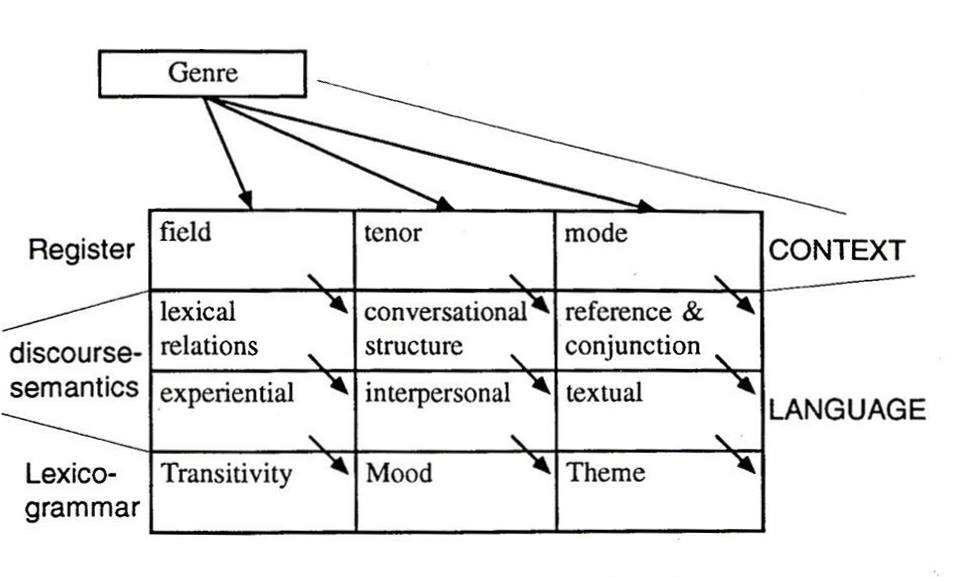
\includegraphics[width=0.85\textwidth]{../images/egginsfixed.jpg}
		\label{fig:eggins}
		\caption{Strata and metafunctions of language (from Eggins, 2004)}
		\end{figure}

		Three key factors informed our decision to adopt the SFL framework for our study. First, in contrast to most mainstream grammars, SFL conceptualises lexis and grammar as a different ends of the same system: lexis is the most delicate realisation of grammar \cite<see>{hasan_grammarians_1987}. Such a conceptualisation, we believe, is vital to an investigation of the behaviour of a concept in a large text corpus, as much of this behaviour will indeed be grammatical. Accordingly, in this study, automated parsing of corpus texts is used to carry out (often simultaneous) searches of both grammar and lexis.

		The second benefit of SFL to our research aims is that SFL is explicitly designed as a framework that to make it possible to say meaningful things about how real-world instances of language work to build meanings and perform social functions. It is thus an \emph{appliable linguistics}, built to `empower researchers to undertake projects of investigation and intervention in many contexts that are critical to the workings of communities and the quality of human life' \cite[p.~437]{matthiessen_applying_2013}.

		Finally, SFL contains the best-articulated means of systematically connecting instantiated lexicogrammatical units (i.e. wordings) to the more abstract stratum of discourse-semantics (i.e. meanings) \cite{eggins_analysing:_2004}. On the strength of this link is the whole endeavour of corpus-discourse research predicated: absent a systematic connection of these two planes of abstraction, corpus-assisted discourse studies lose much of their explanatory power, and corpus-informed discourse research becomes a contradiction in terms.

	\section{Risk words and the systemic functional grammar}

		Perhaps the most laudable achievement of SFL is the ability of its grammar (admitted even by critics, e.g. \citeNP{widdowson_text_2008}) to connect the three kinds of meanings to distinct components of lexicogrammar in consistent, stable ways. Interpersonal meanings are made through the \textbf{mood system}, including features such as \emph{modality} and \emph{modulation}. Textual meanings are made through the use of \textbf{systems of reference and conjunction} between and within clauses. Experiential meanings are made via the \textbf{transitivity system} (predicators, their subjects and object arguments, and adjuncts, in more mainstream grammars). This latter system is of most interest to us.\endnote{Though role relationships between journalists and their readership have undergone significant shifts (especially since the popularisation of online news), charting these changes falls largely outside the scope of this project.}~
		In SFL, transitivity analysis of a clause involves breaking it down into its \emph{process}, \emph{participants} and \emph{circumstances}, realised by verbal groups, nominal groups and adverbials/prepositional phrases, respectively. Most central is the process, whose head (the rightmost verb in a verbal group), may be grouped into five types: \textbf{material processes} (doing and happening: \emph{Risk declined}), \textbf{mental processes} (thinking: \emph{She thought it risky}), \textbf{verbal processes} (saying: \emph{We talked about the risks}), \textbf{existential processes} (\emph{There are risks}) and \textbf{relational processes} (being and having: \emph{It seemed risk-free}). Each type has different configurations of possible participants: mental processes have \emph{Senser} and \emph{Phenomenon} (the sensed); material processes generally have an \emph{Actor}, in subject position, with optional participants such as \emph{Goal}, \emph{Range} and \emph{Beneficiary}. Circumstances (e.g. `\emph{this week}' in Figure \ref{fig:transannotation}) provide specifications such as the manner, extent or location of the process. Circumstances are more syntactically flexible, in that they are often able to be placed in a number of positions within the clause.

			\begin{figure}[htb]
			\centering \small \onehalfspacing
    			\begin{tabularx}{0.75\textwidth}{|l|l|X|X|X|}
    			\hline
    			\emph{But}     & \emph{the bang of the gavel}             & \emph{can hold}          & \emph{risk} & \emph{for novices}          \\ \hline
    			~ & Participant: & Process: & Participant: & Circumstance:  \\
    			    			~ & Carrier & Relational \mbox{attributive} & Attribute &  Extent \\ \hline
    			\end{tabularx}
			\caption{Transitivity analysis of a clause}
			    			\label{fig:transannotation}
			\end{figure}

		An important caveat remains. SFL considers each kind of meaning as having a \emph{congruent} realisation in the lexicogrammar---participants are congruently nominal; qualities as congruently adjectival. Aside from simply using native speaker intuition tests, SFL theorists argue that congruent forms often can be identified by their \emph{typicality} and their \emph{unmarkedness}: congruent realisations are expected to be more frequent in the language as a whole, and to involve fewer derivational morphemes (\emph{nation} as a thing is less inflected than the quality, \emph{national}) (Lassen, 2003). That said, as \citeA[p.~?]{halliday_introduction_2004} explain, `it is by no means easy to decide what are metaphorical and what are congruent forms'. \emph{Risk} is in itself a good example of a concept that straddles the terrain between participant, process and quality.

		%Lassen: Imperative readings of grammatical metaphor

		Incongruent choices, however, are also common in many kinds of texts, carrying a `very considerable semantic load' \cite[p.~?]{halliday_introduction_2004}. First, through \emph{grammatical metaphor}, semantic processes may be realised grammatically as participants (`I accepted \emph{the invitation}') for the purpose of packing more information into clauses---a key feature of written journalistic text \cite{simon-vandenbergen_grammatical_2003}. Furthermore, similar meanings may be made at different ranks/strata of language: `a good risk' and `a risk is good' communicate the same positive appraisal of the same participant, but at different levels (group/phrase level via adjectival modification in the first example; clause level via relational ascription in the second). Incongruence poses serious challenges for corpus linguistic studies of discourse, as it limits our ability to locate, for example, all the ways in which risk is evaluated, graded or judged. This issue is exacerbated if, in line with SFL theory, we consider all lexicogrammatical choices to be meaningful and purposive, including the author's decision to invoke an incongruent form \cite<as in>{eggins_introduction_2004}. In some cases, rank-shifted meanings may be found using increasingly complicated lexicogrammatical search queries (see Figure \ref{fig:glossed} for an example). Automatic location of some other cases remain at this point beyond our capabilities: in appraisal at the level of clause-complex (`\emph{I see a risk---it's a big one}') extremely complex grammatical searches would be needed to first recover the identity of \emph{it} and \emph{one} as \emph{a risk}, before we could automatically determine that the risk is being semantically modified by \emph{big}. Accordingly, our analysis is limited to group/phrase and clausal levels, with meanings made via the clause complex excluded.

	\begin{table}
	  \centering
		  \begin{tabular}{|l|}
		  \hline
		  Clause complex \\ \hline
		  Clause		 \\ \hline
		  Group/phrase   \\ \hline
		  Word		   \\ \hline
		  Morpheme	   \\ \hline
		  \end{tabular}
		  \caption{Rank Scale in SFL}
		  \label{tab:rank}
	  \end{table}

		\subsection{Risk and the experiential metafunction}

			%Risk, as well as the French \emph{risque}, have a long history of use as both noun and verb \cite{hamilton_meanings_2007}, though otherwise its etymology is largely unknown. The lack of derivational morphemes makes it difficult to tell whether risk is congruently a process or a participant. Accordingly, we do not assume it to be congruently either.

			We situate our analysis of risk words predominantly within the experiential realm of meaning. At the most abstracted level of this dimension of language, we are interested in changes in the field of discourse in which risk as a concept is instantiated: \emph{has risk shifted, as per key claims of sociological theory, from international relations toward population health?} Then, within these fields, we are interested in the constellations of happenings in which risk may play a role: \emph{when risk is a process, what participants are involved? When risk is a participant, what is it a participant in, and with whom? And when risk is part of a modifier, what kind of participants and processes does it modify, and how?} Through categorisation of the kinds of fields in which risk appears, as well as the kind of participants who are positioned as riskers, risked things and potential harms, we can then empirically test the claims of influential sociological examination of risk discourse. %(See Table \ref{tab:claims}).

			~\ \todo[inline,color=green!40]{\noindent Either this needs to be expanded, or the mood description contracted...}
			

				%ARGUABILITY \cite[p.~271{matthiessen_combining_2002}, \cite[p.~115]{halliday_introduction_2004}.
				%PP as mini relational clause: \cite{matthiessen_lexicogrammatical_1995}

				%\cite{halliday_grammar_1996}

	\subsection{Risk and the interpersonal function: arguability}

		Though our analysis is for the most part concerned with experiential meanings (via the Transitivity system), some aspects of interpersonal meanings (via the Mood system) are also relevant. Accordingly, a brief sketch of the mood system is required.

		In SFL, the Mood system is used to give and request information (semiotic commodities) or goods and services (material commodities). Congruently, interrogatives request information, and imperatives request goods and services. Declaratives provide information. Being by far the most common mood type in news discourse, our analysis is focussed on the structure of the declarative. A declarative clause contains a Mood Block, which contains a Subject and Finite (see Figure \ref{fig:moodannotation}). Locating the constituents of the Mood Block is simple: if a tag question is added to this declarative (\emph{the bang \dots can hold risks \dots, can't it?}), the tag picks up the Subject and the Finite (with polarity reversed).

		Modality, also a component of the interpersonal metafunction, concerns modification of propositions with speaker judgements.\endnote{The corpus contained too few modalised risk predicators for analysis of longitudinal change in modalisation.}
		Prototypically, Modality is expressed through modal auxiliaries in the Finite position (\emph{I can/should/might go}). Through Modality, speakers `construe the region of uncertainty between yes and no' \cite[p.~147]{halliday_introduction_2004}. In Figure \ref{fig:moodannotation}, for example, \emph{hold} is modalised through \emph{can} in order to express the author's judgement as to the possibility of the banging of the gavel holding risks.

			\begin{figure}[htb]
			\centering \footnotesize \onehalfspacing
    			\addvbuffer[12pt 8pt]{\begin{tabularx}{0.75\textwidth}{|l|l|l|X|X|X|}
    			\hline
    			\emph{But}     & \emph{the bang of the gavel}             & \emph{can} & \emph{hold}          & \emph{risk} & \emph{for novices}          \\ \hline
    			~ 				& 		Subject     						& Finite 		& Predicator 		  & Complement & Adjunct  \\ \cline{2-6}
    			~ 				& 		 \multicolumn{2}{c|}{MOOD} 							& \multicolumn{3}{c|}{RESIDUE} \\ \hline
    			\end{tabularx}}
			\caption{Mood analysis of a clause}
			    			\label{fig:moodannotation}
			\end{figure}

		%how does this bit work: %Modalised declaratives to some extent pattern with the provision of goods and services, either via de(\emph{I can/will/shall visit you}) or speech acts, (\emph{I pronounce you husband and wife})

		At a greater level of abstraction, these Mood and Modality choices are responsible for the construction of role relationships between interactants: where interactants are of equal status (i.e. friends chatting at a cafe), similar overall frequencies in mood choices for each interactant may be observed. In a situation with interactants of less equal status, mood choice frequencies may vary more widely for the different participants: in a typical interaction between a professor and an undergraduate, only the professor is likely to use imperatives to issue commands. Importantly, as with experiential meanings, incongruence may occur, though the motivation for incongruence is an interpersonal one, such as politeness or face saving (\emph{Shut the door!/Could you shut the door?}). For us, however, this kind of incongruence does not pose the same level of challenge as experiential incongruence, as print news journalism as a genre rarely commands or requests information from the reader, and as the faces of both writer and reader are rarely under threat.

		We are interested in Mood mostly because Mood is the system through which \emph{arguability} of propositions is mediated. In SFL, arguability is used to denote the relative ease of challenging or refuting a proposition, and thus, the level of implicitness of a meaning made about the world.

		Chiefly, arguability rests in the two components in the Mood Block---the Finite and the Subject. To make a proposition arguable, it must be grounded in time and space, or to a speaker judgement of its validity. These are the two potential functions of the Finite. Locating a proposition within time and space is done through adding primary tense (\emph{lives were risked}). Meanings are linked to speaker judgements through modality (\emph{lives might be risked}) \cite[p.~116]{halliday_introduction_2004}. In either case, the Finite grounds the proposition with reference to the current exchange being undertaken by the interactants. Primary tense situates a proposition according to what is present at the time the utterance is made---it indicates `the time relative to now' \cite[p.~116]{halliday_introduction_2004}. Modality either expresses an assessment of the validity (probability, certainty, obligation, etc.) of a proposition (\emph{it might/will/must happen}) or, in an interrogative, invites the addressee to make this assessment (\emph{might/will/must it happen?}).

		The Subject is the second component of arguability. Semantically, SFL treats the Subject as `something by reference to which the proposition can be affirmed or denied' \cite[p.~117]{halliday_introduction_2004}. In the contexts of proposals and commands, it is the one who is supposed to perform the action (\emph{Shut the door, will you?}/\emph{I'll speak to her, shall I?}). In the case of declarative information provision, the Subject is the thing upon propositional validity rests. In \emph{the bang of the gavel can hold risk for novices}, for example, a refutation still requires a coherent Subject and Finite, while the Residue is only required if it is the challenged component:

        \begin{quote}
        \small
        \begin{enumerate}	\setlength\itemsep{-0.5em}
		\item No, \emph{it should} hold risks (refuting Modal Finite/speaker judgement)
		\item No, but \emph{a handshake can} (refuting Subject)
		\item No, but \emph{it can} hold excitement (refuting Complement)
		\item No, but \emph{it can} for experts (refuting Complement)
        \end{enumerate}
        \end{quote}
		%
		Thus, the Mood Block is the most arguable part of a proposition---`it carries the burden of the clause as an interactive event' \cite[p.~118]{halliday_introduction_2004}. The steps an interlocutor needs to take to deny the validity of a meaning are fewest when the disagreement concerns the composition of the Mood Block. Meanings made within Complements and Adjuncts, or within groups or phrases, are more implicit: they support, rather than enact, meanings made within the Mood Block \cite{matthiessen_combining_2002}.

		%In this investigation, as in \citeA{matthiessen_lexicogrammatical_1995,matthiessen_combining_2002}, arguablity is also operationalised as a cline, with meanings ranging from very arguable to very inarguable based on the rank at which they are made.  Heads of processes and participants are arguable. Internal modification of groups, especially within subordinate clauses, are likely to be very inarguable. Circumstances---that is, PPs modifying the process---sit in the middle of the two extremes.




		%\begin{table}
		%\centering
		%\footnotesize
   		%\begin{tabular}{|l|l|l|l||l|}
		%\cline{1-4}
		%\multicolumn{2}{|c|}{\textbf{Metafunctions}} & \multicolumn{2}{c||}{\textbf{Lexicogrammar}} & \multicolumn{1}{c}{~} \\ \hline
   		% \emph{Experiential}  & \emph{Interpersonal}   & \emph{Rank scale}         & \emph{Group structure} & \emph{Arguability} \\ \hline
   		% Process       & Finite, Subject & Clause       & Head            & \textbf{Higher}                   \\ \hline
    		%Participant(s)  & Complement      & Group/phrase & Modifier        & \textbf{Medium}                 \\ \hline
    		%Circumstances & Adjunct         & Word         & Submodifier     & \textbf{Lower}                    \\ \hline
   		%\end{tabular}
		%\end{table}

			%\begin{table}
	  %\centering
		  %\begin{tabular}{|l|l|}
		  %\hline
		 	%\textbf{Rank scale} & \textbf{Arguability} \\ \hline
		  %%Clause complex & --- \\ \hline
		  %	Clause	 & Very arguable \\ \hline
		  %Group/phrase   & Arguable \\ \hline
		  %Word		   & Somewhat inarguable \\ \hline
		  %Morpheme	   & Very inarguable \\ \hline
		  %\end{tabular}
		  %\caption{Rank scale and arguability as operationalised here}
		  %\label{tab:rankarg}
	  %\end{table}



	  In the context of risk words, this conceptualisation of arguability can be used to empirically examine key sociological claims. Increasing prevalence of risk words generally would mean that risk words have an inbound trajectory in the NYT generally. Increasing risk words within the Mood Block and Predicator positions would indicate that risk is discussed and argued about. A shift from Mood Block to Residue (especially Complement and Adjunct positions) would indicate greater implicitness and inarguability of risk. At the same time, risk words as heads of groups/phrases would indicate greater discussion of risk, while risk words as modifiers would indicate implicitness.

    \begin{table}
    \centering
    \footnotesize
    \begin{tabularx}{.70\textwidth}{|L{.50}|L{.50}|L{2}|}%
    \hline
    \textbf{Role}              & \textbf{Arguability} & \textbf{Example} \\ \hline
    Subject           & Very high   & \emph{For Mobic, the \textbf{risks} of heart attack and stroke rose 37 percent, Dr. Graham's study showed.}       \\ \hline
    Finite\slash Predicator & High        & \emph{But candid talk about job prospects and debt obligations \textbf{risked} the wrath of management, she said.}       \\ \hline
    Complement        & Medium      & \emph{This approach holds some \textbf{risk} for a union boss.}       \\ \hline
    Adjunct           & Low         & \emph{The wire is stretched very tautly, and we are at some significant \textbf{risk} it will snap from overload.}       \\ \hline
    \end{tabularx}
    \caption{Arguability of risk words in differing mood constituents}
    \end{table}

    \begin{table}
    \centering
    \footnotesize
    \begin{tabularx}{.70\textwidth}{|L{.50}|L{.50}|L{2}|}%
    \hline
    \textbf{Role}              & \textbf{Arguability} & \textbf{Example} \\ \hline
    Head           & Higher   & `\emph{So far, pregnancy \textbf{risk} does seem to come with this class of drugs},' Ms. Glynn said.       \\ \hline
    Non-head   & Lower   & \emph{They purchased billions of dollars in \textbf{risky} subprime mortgages.}       \\ \hline
    \end{tabularx}
    \caption{Arguability of risk words as either head or non-head}
    \end{table}

        The ways in which we operationalise the notion of arguability while interrogating the parsed data are outlined in Section \ref{sect:arguability}.

		
	%\section{SFL and news discourse}

		%~\ \todo[inline,color=green!40]{\noindent Still to write ... }

			%\begin{enumerate}
			%\item Situate our research area as `hard news' \cite{gonzalez_rodriguez_tracing_2006}
			%\item Text and context in hard news
			%\item \citeNP{bednarek_evaluation_2006} % http://books.google.com.au/books?hl=en&lr=&id=8nk0BArolPwC&oi=fnd&pg=PR5&dq=%09+Evaluation+in+media+discourse+:+analysis+of+a+newspaper+corpus&ots=IFz58ZksVq&sig=gRPv0070_O31kOYTCwiBKrLC16Q&redir_esc=y#v=onepage&q=Evaluation%20in%20media%20discourse%20%3A%20analysis%20of%20a%20newspaper%20corpus&f=false
			%\item Limitations and points of difference
			%\end{enumerate}
			%}

	\section{SFL and corpus linguistics}

		Methodologically, our study may be characterised as an attempt to combine the systemic functional conceptualisation of language with practices from diachronic corpus linguistic (CL) research. As \citeA{hunston_systemic_2013} notes, SFL and CL share a number of underlying similarities, such as an emphasis on natural language a focus on register/genre as shaping the lexicogrammatical choices made in texts. More fundamentally, both CL and SFL posit that we can learn about these texts through quantification of their various lexical, grammatical and semantic properties. %Less commonly noted are that both SFL and corpus linguistics are probabalistic, and accordingly, both have predictive applications \cite{halliday_corpus_1991}.

		We use SFL and CL in tandem to locate patterns in texts without manual interpretation or categorisation. Sociological insights into key events and movements are then mapped at later stages to observed lexicogrammatical and discourse-semantic change in the behaviour of risk words (challenges in balancing the systemic-functional notion of context-in-text with the use of sociological methods are discussed below). Such an approach is characteristic of the emerging field of \emph{corpus-assisted discourse studies} (CADS). The oft-noted `methodological synergy' of CL and discourse analysis allows researchers a greater degree of empirical and quantitative support for claims, as well as a larger body of examples that can easily be accessed and qualitatively analysed \cite{baker_useful_2008}. In terms of risk, corpus-based methods allow an empirical testing of sociological literature that has tended to invent examples of clauses containing risk words, despite there being little evidence that these phrases are commonly instantiated in general language use \cite{hamilton_meanings_2007}. Research has also tended to conflate risk words with the concept of risk itself, even though the word may not be critical to the experiential meaning of a clause (the \emph{risk management team went for coffee}) and even though the latter is often present without the linguistic instantiation of the former.

		Work within CADS varies chiefly in the extent to which the corpus itself is the focus of the investigation. In \emph{corpus-driven} work, researchers are attempting to demonstrate that the corpus itself contains particular patterns of discourse. Theories are developed inductively according to patterns located in the data. \emph{Corpus-informed} studies, on the other hand, may use the corpus as a body of examples that can be drawn upon in discussion of broader trends in society \cite{baker_useful_2008}. Theories to be tested are developed before the corpus interrogation

		Our study is in the latter domain.\endnote{Though we are focussed on corpus-assisted investigation at present, indeed the dataset under investigation is of size and scope as to be of interest to corpus-driven researchers, language and media specialists, etc., and indeed, such projects are forthcoming.}
		As a diachronic investigation, we can further situate our method within \emph{Modern Diachronic CADS}. As Partington explains, 

		\begin{quote}
		\lbrack MD-CADS\rbrack~ employs relatively large corpora of a parallel structure and content from different moments of contemporary time \dots in order to track changes in modern language usage but also social, cultural and political changes as reflected in language \citeyear[p.~83]{partington_modern_2010}.
		\end{quote}

		\noindent As newspapers are well-structured and archived in digital collections, they have formed a common datasource for CADS. \citeA{johnson_`political_2003-1} investigated shifts in the discursive construction of \emph{political correctness} in German newspapers. \citeA{duguid_newspaper_2010} performed thematic categorisation of the keywords from two collections of digitised newspapers from 1995 and 2005. \citeA{freake_cross-linguistic_2012} focussed on the ideological positioning of French and English in Canadian newspapers. %do these consider current events??

		Ours is not the first corpus-based study of risk. Most well-known is \citeA{fillmore_toward_1992}, who studied the behaviour of risk as both noun and verb in a 25 million word corpus of American English. Ultimately, the authors' aims were lexicographic, rather than discourse-analytic, limiting the usefulness of the study's methods for our purposes. A second key point of difference is the small size and lack of structure of their corpus (though their research was a certainly remarkable and groundbreaking effort at the time of publication). Finally, their study was neither longitudinal, nor designed to connect patterns to social/societal change.

		More recently, \citeA{hamilton_meanings_2007} used a frame semantics approach to understand the behaviour of risk in two corpora: the 56 million word \emph{Collins WordbanksOnline Corpus} (N risk tokens) and the five million word \emph{CANCODE} (235 risk tokens). 
		%Frame semantics is a well-established framework for functional analysis of language. 
		We depart from their methods in five respects. First, they use general corpora, while we used a specialised corpus. Second, our study is diachronic, while theirs is largely monochronic. Third, we differ dramatically in the number of risk words analysed (n/n). Fourth, they relied on collocation (without lemmatisation\endnote{Lemmatisation is the process of counting the base forms of tokens, rather than the token itself. \emph{Taken} would be classified under \emph{take}, for example. While lemmatisation is not \emph{always} the best option, as it can collapse different parts of speech, tense information, etc., it is certainly appropriate when determining the most common predicators, etc.}), while we performed specific queries of the lexicogrammar, using lemmatisation where needed. Sixth, they used frame semantics, while we use SFL (though informed by Filmore and Atkins' \citeyear{fillmore_toward_1992} articulation of the components of the risk frame, as in Figure \ref{fig:fil_atk}). Though these theories have a number of underlying similarities (both are semantically oriented grammars, for example), the two diverge in their treatment of the role of cognition and psychology. While frame semantics argues that lexicogrammatical instantiations are mapped by listeners to preexisting cognitive frames or schemata, SFL is largely silent on the subject of cognition, preferring to map lexicogrammar to external variables of field, tenor and mode.

            \begin{figure}[htb!]
            \centering
            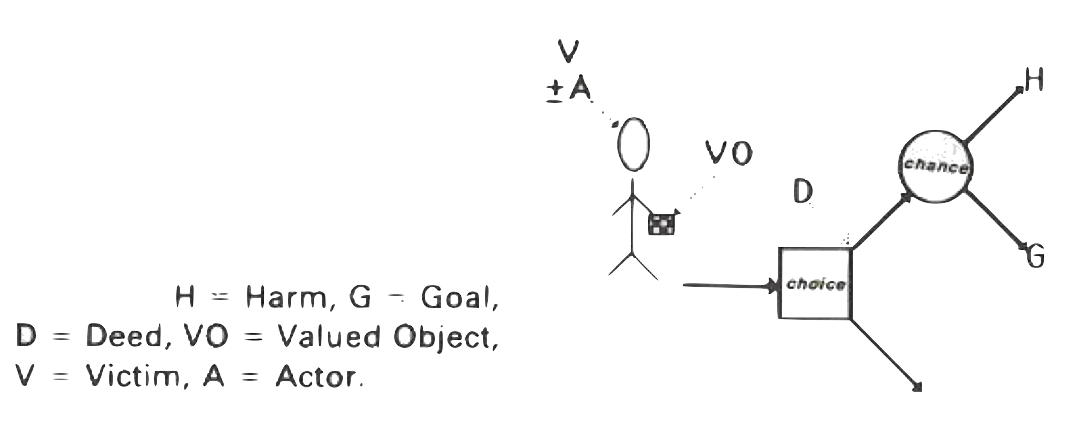
\includegraphics[width=0.6\textwidth]{../images/riskframe.png}
            \caption{Risk frame (from Fillmore \& Atkins, 1992)}
            \label{fig:fil_atk}
            \end{figure}

		%frame semantics vs sfl: http://ucrel.lancs.ac.uk/publications/cl2003/papers/hunston.pdf
		
		%They relied on manual thematic categorisation of concordance lines---something not practical for a corpus containing as many tokens as ours. Their reliance on collocation meant that lists of the closest collocates of risk are not organised by part of speech. This makes it hard to draw meaningful conclusions. Results are also not lemmatised---\emph{is} and \emph{are} are both listed as lower-significance collocates, though had they been classed together with all forms of \emph{be}, \emph{be} may have been demonstrated to play a more important role. Also, their corpus is `balanced', while ours is from a single source.

		Notably, our methodology also departs from typical methods of (MD-)CADS in a few key respects. First, CADS is often lexically-oriented, with techniques such as \textbf{keywording} used as a means of disinterring the `aboutness of a text' \cite{baker_querying_2004} and \textbf{clustering} and \textbf{collocation} used to look for the co-occurrence of lexical items absent any consideration of grammar. \citeA{hunston_systemic_2013} contends that despite a number of areas of overlap, SFL and CL are at odds in the sense that SFL is grammatically oriented while CL is lexically oriented. Though the majority of CADS does indeed focus on lexis, this preoccupation stems more from the relative simplicity of searching for tokens in corpora, compared to grammatical features, than it does from any theoretical motivation.\endnote{We need only to look at the number of lines of code needed to develop an accurate tokeniser and an accurate grammatical structure parser to understand the reasons why lexis appears as the de-facto centre of CL/CADS today}~Accordingly, our use of grammatically parsed data and equal consideration of lexical and grammatical features, though in line with SFL, is against the grain of much contemporary CADS literature.

		The second key difference from mainstream CADS is that we did not rely on typical practices such as keywording, clustering, collocation and the use of stopword lists. Our reasons for avoiding these practices are varied. Keywording we found to be problematic due to its reliance on a reference corpus of general language. The usefulness of this reference corpus is predicated on the idea of corpus balance---that is, the notion that a corpus of texts, if comprised of a wide variety of genres, and if the relative proportion of these texts is akin to their prevalence in culture, may be taken to be representative of language generally \cite{chen_sinica_1996}. As corpus balance is well-acknowledged by CADS practitioners to be only a theoretical ideal (Gries, 2009), we took a different approach. Rather than keywording, we simply counted the base forms of the most common heads of participants, processes and circumstances in each subcorpus. This also liberated us from the arbitrary nature of stopword lists (lists of very common words that are automatically excluded from search results), as most stopwords are determiners, prepositions, conjunctions and so on, which rarely occupy key experiential roles.

		Clustering and collocation, though mainstays of CADS, are also absent in our analysis, as they consider only the co-occurrence of lexical items within a specified (and arbitrary) number of words, and accordingly do not take grammatical relationships into account. As an example, \emph{Men are from Mars, and women are from Venus} would contribute to an understanding of \emph{Mars} and \emph{women} as collocates, regardless of the fact that the experiential meaning of the clause has the opposite meaning. We instead created nuanced search queries capable of drawing on lemma lists and lists of process types (as in Figure \ref{fig:glossed}). This luxury was afforded by grammatical (phrase structure and dependency) annotation of the corpus, as well as the development of scripts for quickly searching lexicogrammar.

		%Quantitative corpus linguistics with R: a practical introduction

		%This was primarily to avoid conflicts between these practices and the theoretical orientation discourse analysis:

			\begin{figure}
			\begin{quote}
			\begin{multicols}{2}
			\begin{verbatim}
			__ >># (/(NP|VP|PP)/ > (VP
			<<# process.relational $ 
			(@NP <<# /(?i)\brisk.?/)))
			\end{verbatim}
			\noindent In relational processes in which a risk word is the Token/Carrier, what is the head of the Value/Attribute?
			\end{multicols}
			\end{quote}
			\caption{\emph{Tregex}-based search query and gloss}
			\label{fig:glossed}
			\end{figure}

			\section{Discourse-semantic areas of interest}

				Our interest is ultimately in discourse-semantic experiential and interpersonal meanings of risk words. The first point of interest is simply the relative frequency of risk words in the NYT generally, and by word class. These areas of interest are at the clausal level. Within experiential meaning, we are interested the relative frequency of risk as a Participant and as a Process, as well as the behaviour of risk when occupying these roles. At the same time, we are interested in meanings made below clause level, within groups and phrases. When risk is a participant or process, we are interested in the ways it is modified. Furthermore, risk itself can be a modifier of participants and processes. Accordingly, we are also interested in both understanding the ways in which this modification happen and finding the participants and processes that risk commonly modifies. Finally, within the interpersonal realm of meaning, we are interested in the arguability of risk words---that is, the extent to which their meaning is symbolically available to negotiation by the writer/reader.

				We can summarise our discourse-semantic interests with the following \ref{lst:num} questions. \emph{In terms of longitudinal change in the NYT,}

				\begin{enumerate}\setlength\itemsep{-0.5em}
					\item \emph{How frequently do risk words appear?}
					\item \emph{Which experiential roles do risk words occupy?}
					\item \emph{Is risk more commonly in the position of experiential subject or experiential object?}
					\item \emph{What processes are involved when risk is a participant?}
					\item \emph{How are participant risks modified?}
					\item \emph{What kinds of risk processes are there, and what are their relative frequencies?}
					\item \emph{When risk is a process, what participants are involved?}
					\item \emph{When risk is a modifier, what are the most common forms?}
					\item \emph{When risk is a modifier, what is being modified?}
					\item \emph{How arguable is risk?} \label{lst:num}
				\end{enumerate}
				%
				These questions are answered in this order in the Findings section. In the Discussion, these answers are synergised in order to perform a broader analysis of discouse-semantic change.

		\section{Lexicogrammatical realisations of discourse-semantic meanings}

			Discourse-semantic meanings are realised in texts by lexicogrammatical patterns. \textbf{Risk as participant} is congruently realised by a risk word at the head of a noun phrase that is an argument of a main verb. Other possible realisations of risk participants are adjectival risk words in participant positions (\emph{The job is risky}) or risk words within prepositional phrases (\emph{Votes were at risk}). SFL also treats prepositional phrases as partially realised relational processes, containing only object arguments. As this is perhaps a controversial analysis within linguistic theory generally, the treatment of risk within PPs is separated from risk as arguments of verbal groups. \textbf{Risk as a process} is congruently realised by a risk word as the main verb of a clause. When risk is instantiated here, we can extract the participants involved in the process. \textbf{Risk as a modifier} is realised by different word classes, depending on what is being modified. Risk can modify participants through pre-head or post-head modification. Analysed in this study\endnote{Modification through embedded clauses (\emph{the children who were at risk}) has been left out for reasons of scope.} are adjectival pre-head modification (\emph{a risky move}), nominal pre-head modification (\emph{risk management}) and post-head modification via a prepositional phrase (\emph{the electorate at risk}). \textbf{Arguability of risk words} can be determined by looking for the functional role of risk words within the Mood system: risk as Subject or Predicator is more arguable than risk as Complement and Adjunct. 

			%Risk can modify either participants or processes. Participants are modifier through pre- or post-head attachments within the nominal group (\emph{a risky decision}; \emph{a man at risk of harm}. Processes are modified by adverbials or by prepositional phrases that attach to the verbal group (\emph{he gambled riskily}; \emph{she told me about the risk}).

			%Risk as a modifier of participant. The first, most congruently, involves the use of risk as an Epithet within an adjectival unit  (e.g. \emph{the risky decision}). Note that this may serve either experiential or interpersonal functions: experiential Epithets are objective properties of the head of the phrase; interpersonal Epithets convey speaker judgements. Also possible is risk as a Classifier nominal classifiers (e.g. \emph{risk management}). Here, the head of the noun is restricted to the provided class. 

			%We can now add lexicogrammatical realisations to our discourse-semantic areas of interest:

				%\begin{enumerate}
					%\item how frequently do risk words appear?
					%\item which functional roles (Participant, Process, Modifier) do risk words occupy?
					%\item Is risk more commonly in the position of experiential subject or experiential object?
					%\item what processes are involved when risk is a subject%\slash object participant?
					%\item when risk is a process, what participants are involved?
					%\item how arguable is risk?
					%\item when risk is a modifier, what are the most common forms?
					%\item when risk is a modifier, what is being modified?
				%\end{enumerate}

			%Risk words may be nominal (\emph{a risk}), verbal (\emph{she risks}), adjectival (\emph{a risky venture}) or, rarely, adverbial (\emph{I riskily decided}).


			%Corpus interrogation proceeded through each of these four categories in a wide array of permutations. In each interrogation, we were interested in either a) counting the total occurrences of a lexicogrammatical pattern in each subcorpus (e.g. \emph{How often is a risk word adjectival?}) or b) listing all words matching a search query by total frequency in each subcorpus (e.g. \emph{Which risk-adjectives occur, and how often?}).

			%\begin{enumerate}[nolistsep]
				%\item Counting the total occurrences of a lexicogrammatical pattern in each subcorpus (e.g. \emph{How often is a risk word adjectival?})
				%\item Listing all words matching a search query by total frequency in each subcorpus (e.g. \emph{Which risk-adjectives occur, and how often?})
			%\end{enumerate}

			The scope of our project necessitated some constraints on the kinds of patterns we analysed. Major constraints included our focussing on experiential meaning, perhaps at the expense of interpersonal meaning. Thus, the analysis contains little consideration of how risk may be operationalised in order to construct writer/reader or newspaper/readership relationships. Also largely unanalysed are the ways in which risk are appraised, judged, and graded in severity. This was mostly due to the lack of available automatic parsers for SFL's appraisal grammar \cite<see>{martin_language_2005}. Finally, queries returning less salient or ambiguous results are omitted from discussion here. Counting the kinds of determiners that occur before a nominal risk (this risk, a risk, the risk) uncovered no particularly interesting patterns, for example.

				%make all queries and results available?

				%MUST CHANGE THESE PARAGRAPHS TO RISK AS PARTICIPANT, PROCESS,


		%\subsection{Dependency querying}

			%\begin{figure}[htb!]
			%\centering
			%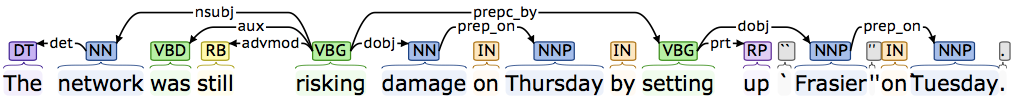
\includegraphics[width=0.75\textwidth]{../images/depparse}
			%\caption{A visualised dependency parse, with \emph{risking} as root}
			%\label{fig:depparse}
			%\end{figure}		

			%\section{Operationalising sociological claims}

			%The discourse-semantic and lexicogrammatical areas of interest can be summarised with regard to related sociological claims.

		      %\begin{table}
		      %\centering
		      %\footnotesize
		      %\begin{tabularx}{1.0\textwidth}{|l|X|X|X|X|}
		      %\hline
		      %\textbf{Author}   & \textbf{Claim}   & \textbf{Discourse-semantic realisations(s)}      & \textbf{Congruent lexicogrammatical realisation(s)}    & \textbf{Example(s)}  \\ \hline
		      %Beck     & Everyday life world characterised by risk    & Common people as increasingly common participants in risk as a process; increasingly localised risked things/potential harms; risk appearing in articles about daily life & Women, children, non-celebrities appearing as heads of nominal groups that are actors in risk processes; Everyday processes and common things appearing as head of verbal and nominal groups that appear after risk processes & \emph{The little girl risked tearing her coat}; \emph{We risked getting rained on/one dollar}; \\ \hline
		      %Giddens  & ~ & ~    & ~       & ~       \\ \hline
		      %Zinn     & ~     & ~      & ~       & ~    \\ \hline
		      %Author x & Increasing focus on risk in health discourse & Medical lexis (diseases, institutions, medications, etc) as increasingly common participants in risk as a process                                                         & Illnesses and risk in nominal compound words; health terminology in modifiers of risk as head of a participant    & \emph{The cancer-risk}; \emph{the risk of heart disease}                                       \\ \hline
		      %Author y & ~     & ~       & ~       & ~      \\ \hline
		      %\end{tabularx}
		      %\caption{Systemic-functional realisations of sociological claims concerning risk discourse}
		      %\label{tab:claims}
		      %\end{table}

			%\subsubsection{Longitudinal trajectory} will be used to refer to a given lexicogrammatical construction increasing in frequency (\emph{inbound trajectory}), becoming less frequent (\emph{outbound trajectory}), or remaining at a similar frequency (\emph{static trajectory}) over time.


%\bibliography{../references/libwin}